% Options for packages loaded elsewhere
\PassOptionsToPackage{unicode}{hyperref}
\PassOptionsToPackage{hyphens}{url}
%
\documentclass[
]{article}
\usepackage{amsmath,amssymb}
\usepackage{iftex}
\ifPDFTeX
  \usepackage[T1]{fontenc}
  \usepackage[utf8]{inputenc}
  \usepackage{textcomp} % provide euro and other symbols
\else % if luatex or xetex
  \usepackage{unicode-math} % this also loads fontspec
  \defaultfontfeatures{Scale=MatchLowercase}
  \defaultfontfeatures[\rmfamily]{Ligatures=TeX,Scale=1}
\fi
\usepackage{lmodern}
\ifPDFTeX\else
  % xetex/luatex font selection
\fi
% Use upquote if available, for straight quotes in verbatim environments
\IfFileExists{upquote.sty}{\usepackage{upquote}}{}
\IfFileExists{microtype.sty}{% use microtype if available
  \usepackage[]{microtype}
  \UseMicrotypeSet[protrusion]{basicmath} % disable protrusion for tt fonts
}{}
\makeatletter
\@ifundefined{KOMAClassName}{% if non-KOMA class
  \IfFileExists{parskip.sty}{%
    \usepackage{parskip}
  }{% else
    \setlength{\parindent}{0pt}
    \setlength{\parskip}{6pt plus 2pt minus 1pt}}
}{% if KOMA class
  \KOMAoptions{parskip=half}}
\makeatother
\usepackage{xcolor}
\usepackage[margin=1in]{geometry}
\usepackage{longtable,booktabs,array}
\usepackage{calc} % for calculating minipage widths
% Correct order of tables after \paragraph or \subparagraph
\usepackage{etoolbox}
\makeatletter
\patchcmd\longtable{\par}{\if@noskipsec\mbox{}\fi\par}{}{}
\makeatother
% Allow footnotes in longtable head/foot
\IfFileExists{footnotehyper.sty}{\usepackage{footnotehyper}}{\usepackage{footnote}}
\makesavenoteenv{longtable}
\usepackage{graphicx}
\makeatletter
\def\maxwidth{\ifdim\Gin@nat@width>\linewidth\linewidth\else\Gin@nat@width\fi}
\def\maxheight{\ifdim\Gin@nat@height>\textheight\textheight\else\Gin@nat@height\fi}
\makeatother
% Scale images if necessary, so that they will not overflow the page
% margins by default, and it is still possible to overwrite the defaults
% using explicit options in \includegraphics[width, height, ...]{}
\setkeys{Gin}{width=\maxwidth,height=\maxheight,keepaspectratio}
% Set default figure placement to htbp
\makeatletter
\def\fps@figure{htbp}
\makeatother
\setlength{\emergencystretch}{3em} % prevent overfull lines
\providecommand{\tightlist}{%
  \setlength{\itemsep}{0pt}\setlength{\parskip}{0pt}}
\setcounter{secnumdepth}{-\maxdimen} % remove section numbering
\usepackage{fontspec}
\setmainfont{NanumGothic}
\ifLuaTeX
  \usepackage{selnolig}  % disable illegal ligatures
\fi
\usepackage{bookmark}
\IfFileExists{xurl.sty}{\usepackage{xurl}}{} % add URL line breaks if available
\urlstyle{same}
\hypersetup{
  pdftitle={Quiz 250317},
  pdfauthor={coop711},
  hidelinks,
  pdfcreator={LaTeX via pandoc}}

\title{Quiz 250317}
\author{coop711}
\date{2025-03-17}

\begin{document}
\maketitle

\section{3주차 데이터 실험
집계}\label{uxc8fcuxcc28-uxb370uxc774uxd130-uxc2e4uxd5d8-uxc9d1uxacc4}

\subsection{실험의 목적}\label{uxc2e4uxd5d8uxc758-uxbaa9uxc801}

3주차 구글 예습 설문지 집계결과를 분석합니다.

Q1\textasciitilde Q6에서는 랜덤화의 효과로 Red, Black 이 얼마나 닮았는지
알아봅니다.

Q7에서는 같은 사안에 대해서 질문 안에 편향된 정보를 담아 넣었을 때 Red,
Black 의 응답이 어떻게 달라지는 지 알아봅니다.

끝으로 제출시간의 분포가 날마다 고른지, Red, Black 간에는 닮았는지
알아봅니다.

\subsubsection{Red, Black을 잘못 표시한
사람들}\label{red-blackuxc744-uxc798uxbabb-uxd45cuxc2dcuxd55c-uxc0acuxb78cuxb4e4}

\begin{longtable}[]{@{}
  >{\raggedright\arraybackslash}p{(\columnwidth - 4\tabcolsep) * \real{0.3611}}
  >{\centering\arraybackslash}p{(\columnwidth - 4\tabcolsep) * \real{0.2778}}
  >{\centering\arraybackslash}p{(\columnwidth - 4\tabcolsep) * \real{0.3056}}@{}}
\toprule\noalign{}
\begin{minipage}[b]{\linewidth}\raggedright
~
\end{minipage} & \begin{minipage}[b]{\linewidth}\centering
Red(구글예습퀴즈)
\end{minipage} & \begin{minipage}[b]{\linewidth}\centering
Black(구글예습퀴즈)
\end{minipage} \\
\midrule\noalign{}
\endhead
\bottomrule\noalign{}
\endlastfoot
\textbf{Red(랜덤화출석부)} & 273 & 5 \\
\textbf{Black(랜덤화출석부)} & 4 & 271 \\
\textbf{계} & 277 & 276 \\
\end{longtable}

랜덤화출석부에 있는 Red, Black 과 실제 구글설문에 올린 Red, Black 이
다른 사람들의 수효는 9명입니다.

Red를 Black 이라고 한 사람이 5명, Black 을 Red 라고 한 사람이 4명입니다.

두 가지 방법으로 분석합니다.

우선 Red, Black 을 잘못 선택한 9명을 랜덤하게 둘로 나누면 어느 한 쪽
집단에 들어갈 기대인원은 9명을 둘로 나눈 4.5(명)이고, 표준오차는 9의
제곱근에 1/2을 곱해 준 1.5명이 됩니다.

실제로 Red를 Black 이라고 한 사람수, 5명이나 Black 을 Red 라고 한
사람수, 4명은 기대인원으로부터 표준오차 범위 안에 아주 잘 들어갑니다.

두 번째 분석 방법은 확률을 계산해 보는 것입니다.

Red, Black 을 잘못 선택한 9명을 랜덤하게 둘로 나눌 때, 실제로 관찰된 5명
이상이나 4명이하로 잘못 선택한 사람수가 나올 가능성은 얼마나 되는가
입니다.

이 경우 공평한 동전던지기를 확률 법칙으로 표현한 이항분포로부터 계산할
수 있습니다.

시행횟수가 9이고 한 번 시행에서 성공확률이 1/2 인 이항분포에서
성공횟수가 4이하이거나 5이상을 관찰할 확률은 1입니다.

공평한 동전 던지기에서 앞면이 4개 이하 나오는 확률은 5개 이상 나오는
확률과 같기 때문에 사실상 한쪽만 계산해서 2배 해 주면 됩니다.

이 값을 p-value 라고 하는데, p-value가 0.05보다 작을 때
\textbf{통계적으로 유의한 차이를 관찰}하였다고 말합니다.

즉, 공평한 동전을 던지는 것과 같은 과정이라고 가정하였을 때 실제로
관찰된 값들이 가정으로부터 얼마나 떨어져 있는지를 표현한 것입니다.

0.05, 즉 1/20은 이런 실험을 스무 번 정도 반복하면 1번 나올 정도로 드문
사건을 의미합니다.

즉 가정이 타당하다면 나오기 힘든 결과라는 것입니다.

그런데 Red, Black 을 잘못 표시한 사람들의 분포에서 관찰된 p-value 는
0.05와는 비교도 안될 정도로 큰 값입니다.

따라서 두 집단이 랜덤화 효과가 작동하여 \textbf{통계적으로 유의한 차이를
보이지 않는다}고 할 수 있습니다.

\subsubsection{응답인원의 Red,
Black}\label{uxc751uxb2f5uxc778uxc6d0uxc758-red-black}

Red 로 응답한 인원은 277명, Black 에 응답한 인원은 276명입니다.

전체 응답인원 553 명을 랜덤하게 둘로 나눌 때 어느 한 쪽의 기대인원은
전체 응답인원의 절반인 276.5명이고, 표준오차는 전체 응답인원의 제곱근에
1/2을 곱해 준 11.8 명입니다.

따라서 Red, Black 각 그룹에 관찰된 인원은 기대인원으로부터 표준오차 범위
안에 들어갑니다.

\subsection{Q1. 국세와 지방세
비중}\label{q1.-uxad6duxc138uxc640-uxc9c0uxbc29uxc138-uxbe44uxc911}


\includegraphics[width=0.75\linewidth]{./pics/Quiz230315_Q1}

\subsubsection{국세와 지방세
비중(집계표)}\label{uxad6duxc138uxc640-uxc9c0uxbc29uxc138-uxbe44uxc911uxc9d1uxacc4uxd45c}

\begin{longtable}[]{@{}
  >{\raggedright\arraybackslash}p{(\columnwidth - 12\tabcolsep) * \real{0.1667}}
  >{\raggedleft\arraybackslash}p{(\columnwidth - 12\tabcolsep) * \real{0.1111}}
  >{\raggedleft\arraybackslash}p{(\columnwidth - 12\tabcolsep) * \real{0.1111}}
  >{\raggedleft\arraybackslash}p{(\columnwidth - 12\tabcolsep) * \real{0.1111}}
  >{\raggedleft\arraybackslash}p{(\columnwidth - 12\tabcolsep) * \real{0.1111}}
  >{\raggedleft\arraybackslash}p{(\columnwidth - 12\tabcolsep) * \real{0.1111}}
  >{\centering\arraybackslash}p{(\columnwidth - 12\tabcolsep) * \real{0.1111}}@{}}
\toprule\noalign{}
\begin{minipage}[b]{\linewidth}\raggedright
~
\end{minipage} & \begin{minipage}[b]{\linewidth}\raggedleft
78:22
\end{minipage} & \begin{minipage}[b]{\linewidth}\raggedleft
77:23
\end{minipage} & \begin{minipage}[b]{\linewidth}\raggedleft
76:24
\end{minipage} & \begin{minipage}[b]{\linewidth}\raggedleft
75:25
\end{minipage} & \begin{minipage}[b]{\linewidth}\raggedleft
74:26
\end{minipage} & \begin{minipage}[b]{\linewidth}\centering
계
\end{minipage} \\
\midrule\noalign{}
\endhead
\bottomrule\noalign{}
\endlastfoot
\textbf{Red} & 16 & 35 & 45 & 29 & 152 & 277 \\
\textbf{Black} & 16 & 33 & 55 & 23 & 149 & 276 \\
\textbf{계} & 32 & 68 & 100 & 52 & 301 & 553 \\
\end{longtable}

\begin{longtable}[]{@{}
  >{\raggedleft\arraybackslash}p{(\columnwidth - 4\tabcolsep) * \real{0.2361}}
  >{\raggedleft\arraybackslash}p{(\columnwidth - 4\tabcolsep) * \real{0.0694}}
  >{\raggedleft\arraybackslash}p{(\columnwidth - 4\tabcolsep) * \real{0.1389}}@{}}
\caption{Pearson's Chi-squared test: \texttt{.}}\tabularnewline
\toprule\noalign{}
\begin{minipage}[b]{\linewidth}\raggedleft
Test statistic
\end{minipage} & \begin{minipage}[b]{\linewidth}\raggedleft
df
\end{minipage} & \begin{minipage}[b]{\linewidth}\raggedleft
P value
\end{minipage} \\
\midrule\noalign{}
\endfirsthead
\toprule\noalign{}
\begin{minipage}[b]{\linewidth}\raggedleft
Test statistic
\end{minipage} & \begin{minipage}[b]{\linewidth}\raggedleft
df
\end{minipage} & \begin{minipage}[b]{\linewidth}\raggedleft
P value
\end{minipage} \\
\midrule\noalign{}
\endhead
\bottomrule\noalign{}
\endlastfoot
1.779 & 4 & 0.7763 \\
\end{longtable}

Q1의 집계 결과가 Red, Black 간에 통계적으로 유의한 차이가 있는지
알아보기 위하여 카이제곱 테스트를 수행하였습니다.

그 결과 카이제곱 통계량은 1.78, 자유도는 4 , p-value 는 0.7763이므로
Red, Black 간에 통계적으로 유의한 차이를 보이지 않습니다.

실제로 닮은 게 느껴집니까?

\subsubsection{국세와 지방세
비중(\%)}\label{uxad6duxc138uxc640-uxc9c0uxbc29uxc138-uxbe44uxc911}

\begin{longtable}[]{@{}
  >{\raggedleft\arraybackslash}p{(\columnwidth - 10\tabcolsep) * \real{0.1111}}
  >{\raggedleft\arraybackslash}p{(\columnwidth - 10\tabcolsep) * \real{0.1111}}
  >{\raggedleft\arraybackslash}p{(\columnwidth - 10\tabcolsep) * \real{0.1111}}
  >{\raggedleft\arraybackslash}p{(\columnwidth - 10\tabcolsep) * \real{0.1111}}
  >{\raggedleft\arraybackslash}p{(\columnwidth - 10\tabcolsep) * \real{0.1111}}
  >{\centering\arraybackslash}p{(\columnwidth - 10\tabcolsep) * \real{0.1111}}@{}}
\toprule\noalign{}
\begin{minipage}[b]{\linewidth}\raggedleft
78:22
\end{minipage} & \begin{minipage}[b]{\linewidth}\raggedleft
77:23
\end{minipage} & \begin{minipage}[b]{\linewidth}\raggedleft
76:24
\end{minipage} & \begin{minipage}[b]{\linewidth}\raggedleft
75:25
\end{minipage} & \begin{minipage}[b]{\linewidth}\raggedleft
74:26
\end{minipage} & \begin{minipage}[b]{\linewidth}\centering
계
\end{minipage} \\
\midrule\noalign{}
\endhead
\bottomrule\noalign{}
\endlastfoot
5.8 & 12.3 & 18.1 & 9.4 & 54.4 & 100.0 \\
\end{longtable}

정답률은 Red, Black 을 합하여 계산하는데, 54.4(\%) 입니다.

\subsection{Q2. 조세부담률}\label{q2.-uxc870uxc138uxbd80uxb2f4uxb960}


\includegraphics[width=0.75\linewidth]{./pics/Quiz230315_Q2}

\subsubsection{조세부담률(집계표)}\label{uxc870uxc138uxbd80uxb2f4uxb960uxc9d1uxacc4uxd45c}

\begin{longtable}[]{@{}
  >{\raggedright\arraybackslash}p{(\columnwidth - 12\tabcolsep) * \real{0.1667}}
  >{\raggedleft\arraybackslash}p{(\columnwidth - 12\tabcolsep) * \real{0.0833}}
  >{\raggedleft\arraybackslash}p{(\columnwidth - 12\tabcolsep) * \real{0.0833}}
  >{\raggedleft\arraybackslash}p{(\columnwidth - 12\tabcolsep) * \real{0.0833}}
  >{\raggedleft\arraybackslash}p{(\columnwidth - 12\tabcolsep) * \real{0.0833}}
  >{\raggedleft\arraybackslash}p{(\columnwidth - 12\tabcolsep) * \real{0.0833}}
  >{\centering\arraybackslash}p{(\columnwidth - 12\tabcolsep) * \real{0.0833}}@{}}
\toprule\noalign{}
\begin{minipage}[b]{\linewidth}\raggedright
~
\end{minipage} & \begin{minipage}[b]{\linewidth}\raggedleft
10\%
\end{minipage} & \begin{minipage}[b]{\linewidth}\raggedleft
15\%
\end{minipage} & \begin{minipage}[b]{\linewidth}\raggedleft
20\%
\end{minipage} & \begin{minipage}[b]{\linewidth}\raggedleft
25\%
\end{minipage} & \begin{minipage}[b]{\linewidth}\raggedleft
30\%
\end{minipage} & \begin{minipage}[b]{\linewidth}\centering
계
\end{minipage} \\
\midrule\noalign{}
\endhead
\bottomrule\noalign{}
\endlastfoot
\textbf{Red} & 6 & 28 & 223 & 17 & 3 & 277 \\
\textbf{Black} & 7 & 24 & 221 & 19 & 5 & 276 \\
\textbf{계} & 13 & 52 & 444 & 36 & 8 & 553 \\
\end{longtable}

\begin{longtable}[]{@{}
  >{\raggedleft\arraybackslash}p{(\columnwidth - 4\tabcolsep) * \real{0.2361}}
  >{\raggedleft\arraybackslash}p{(\columnwidth - 4\tabcolsep) * \real{0.0694}}
  >{\raggedleft\arraybackslash}p{(\columnwidth - 4\tabcolsep) * \real{0.1389}}@{}}
\caption{Pearson's Chi-squared test: \texttt{.}}\tabularnewline
\toprule\noalign{}
\begin{minipage}[b]{\linewidth}\raggedleft
Test statistic
\end{minipage} & \begin{minipage}[b]{\linewidth}\raggedleft
df
\end{minipage} & \begin{minipage}[b]{\linewidth}\raggedleft
P value
\end{minipage} \\
\midrule\noalign{}
\endfirsthead
\toprule\noalign{}
\begin{minipage}[b]{\linewidth}\raggedleft
Test statistic
\end{minipage} & \begin{minipage}[b]{\linewidth}\raggedleft
df
\end{minipage} & \begin{minipage}[b]{\linewidth}\raggedleft
P value
\end{minipage} \\
\midrule\noalign{}
\endhead
\bottomrule\noalign{}
\endlastfoot
1.003 & 4 & 0.9094 \\
\end{longtable}

Q2의 집계 결과가 Red, Black 간에 통계적으로 유의한 차이가 있는지
알아보기 위하여 카이제곱 테스트를 수행하였습니다.

그 결과 카이제곱 통계량은 1.003, 자유도는 4, p-value 는 0.9094이므로
Red, Black 간에 통계적으로 유의한 차이를 보이지 않습니다.

실제로 닮은 게 느껴집니까?

\subsubsection{조세부담률(\%)}\label{uxc870uxc138uxbd80uxb2f4uxb960}

\begin{longtable}[]{@{}
  >{\raggedleft\arraybackslash}p{(\columnwidth - 10\tabcolsep) * \real{0.0833}}
  >{\raggedleft\arraybackslash}p{(\columnwidth - 10\tabcolsep) * \real{0.0833}}
  >{\raggedleft\arraybackslash}p{(\columnwidth - 10\tabcolsep) * \real{0.0972}}
  >{\raggedleft\arraybackslash}p{(\columnwidth - 10\tabcolsep) * \real{0.0833}}
  >{\raggedleft\arraybackslash}p{(\columnwidth - 10\tabcolsep) * \real{0.0833}}
  >{\centering\arraybackslash}p{(\columnwidth - 10\tabcolsep) * \real{0.1111}}@{}}
\toprule\noalign{}
\begin{minipage}[b]{\linewidth}\raggedleft
10\%
\end{minipage} & \begin{minipage}[b]{\linewidth}\raggedleft
15\%
\end{minipage} & \begin{minipage}[b]{\linewidth}\raggedleft
20\%
\end{minipage} & \begin{minipage}[b]{\linewidth}\raggedleft
25\%
\end{minipage} & \begin{minipage}[b]{\linewidth}\raggedleft
30\%
\end{minipage} & \begin{minipage}[b]{\linewidth}\centering
계
\end{minipage} \\
\midrule\noalign{}
\endhead
\bottomrule\noalign{}
\endlastfoot
2.4 & 9.4 & 80.3 & 6.5 & 1.4 & 100.0 \\
\end{longtable}

정답률은 Red, Black 을 합하여 계산하는데, 80.3(\%) 입니다.

\subsection{Q3. OECD
국민부담률}\label{q3.-oecd-uxad6duxbbfcuxbd80uxb2f4uxb960}

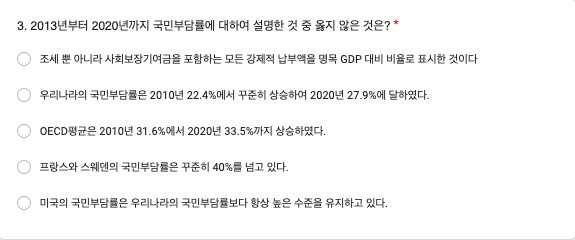
\includegraphics[width=0.75\linewidth]{./pics/Quiz230315_Q3}

\subsubsection{OECD
국민부담률(집계표)}\label{oecd-uxad6duxbbfcuxbd80uxb2f4uxb960uxc9d1uxacc4uxd45c}

\begin{longtable}[]{@{}
  >{\raggedright\arraybackslash}p{(\columnwidth - 12\tabcolsep) * \real{0.0663}}
  >{\centering\arraybackslash}p{(\columnwidth - 12\tabcolsep) * \real{0.1823}}
  >{\centering\arraybackslash}p{(\columnwidth - 12\tabcolsep) * \real{0.1823}}
  >{\centering\arraybackslash}p{(\columnwidth - 12\tabcolsep) * \real{0.1713}}
  >{\centering\arraybackslash}p{(\columnwidth - 12\tabcolsep) * \real{0.1823}}
  >{\centering\arraybackslash}p{(\columnwidth - 12\tabcolsep) * \real{0.1823}}
  >{\centering\arraybackslash}p{(\columnwidth - 12\tabcolsep) * \real{0.0331}}@{}}
\toprule\noalign{}
\begin{minipage}[b]{\linewidth}\raggedright
~
\end{minipage} & \begin{minipage}[b]{\linewidth}\centering
조세 뿐 아니라 사회보장기여금을 포함하는 모든 강제적 납부액을 명목 GDP
대비 비율로 표시한 것이다
\end{minipage} & \begin{minipage}[b]{\linewidth}\centering
우리나라의 국민부담률은 2010년 22.4\%에서 꾸준히 상승하여 2020년
27.9\%에 달하였다.
\end{minipage} & \begin{minipage}[b]{\linewidth}\centering
OECD평균은 2010년 31.6\%에서 2020년 33.5\%까지 상승하였다.
\end{minipage} & \begin{minipage}[b]{\linewidth}\centering
프랑스와 스웨덴의 국민부담률은 꾸준히 40\%를 넘고 있다.
\end{minipage} & \begin{minipage}[b]{\linewidth}\centering
미국의 국민부담률은 우리나라의 국민부담률보다 항상 높은 수준을 유지하고
있다.
\end{minipage} & \begin{minipage}[b]{\linewidth}\centering
계
\end{minipage} \\
\midrule\noalign{}
\endhead
\bottomrule\noalign{}
\endlastfoot
\textbf{Red} & 11 & 40 & 16 & 12 & 198 & 277 \\
\textbf{Black} & 8 & 32 & 18 & 19 & 199 & 276 \\
\textbf{계} & 19 & 72 & 34 & 31 & 397 & 553 \\
\end{longtable}

\begin{longtable}[]{@{}
  >{\raggedleft\arraybackslash}p{(\columnwidth - 4\tabcolsep) * \real{0.2361}}
  >{\raggedleft\arraybackslash}p{(\columnwidth - 4\tabcolsep) * \real{0.0694}}
  >{\raggedleft\arraybackslash}p{(\columnwidth - 4\tabcolsep) * \real{0.1389}}@{}}
\caption{Pearson's Chi-squared test: \texttt{.}}\tabularnewline
\toprule\noalign{}
\begin{minipage}[b]{\linewidth}\raggedleft
Test statistic
\end{minipage} & \begin{minipage}[b]{\linewidth}\raggedleft
df
\end{minipage} & \begin{minipage}[b]{\linewidth}\raggedleft
P value
\end{minipage} \\
\midrule\noalign{}
\endfirsthead
\toprule\noalign{}
\begin{minipage}[b]{\linewidth}\raggedleft
Test statistic
\end{minipage} & \begin{minipage}[b]{\linewidth}\raggedleft
df
\end{minipage} & \begin{minipage}[b]{\linewidth}\raggedleft
P value
\end{minipage} \\
\midrule\noalign{}
\endhead
\bottomrule\noalign{}
\endlastfoot
3.062 & 4 & 0.5476 \\
\end{longtable}

Q3의 집계 결과가 Red, Black 간에 통계적으로 유의한 차이가 있는지
알아보기 위하여 카이제곱 테스트를 수행하였습니다.

그 결과 카이제곱 통계량은 3.062, 자유도는 4, p-value 는 0.5476이므로
Red, Black 간에 통계적으로 유의한 차이를 보이지 않습니다.

실제로 닮은 게 느껴집니까?

\subsubsection{OECD
국민부담률(\%)}\label{oecd-uxad6duxbbfcuxbd80uxb2f4uxb960}

\begin{longtable}[]{@{}
  >{\centering\arraybackslash}p{(\columnwidth - 10\tabcolsep) * \real{0.1930}}
  >{\centering\arraybackslash}p{(\columnwidth - 10\tabcolsep) * \real{0.1930}}
  >{\centering\arraybackslash}p{(\columnwidth - 10\tabcolsep) * \real{0.1813}}
  >{\centering\arraybackslash}p{(\columnwidth - 10\tabcolsep) * \real{0.1930}}
  >{\centering\arraybackslash}p{(\columnwidth - 10\tabcolsep) * \real{0.1930}}
  >{\centering\arraybackslash}p{(\columnwidth - 10\tabcolsep) * \real{0.0468}}@{}}
\toprule\noalign{}
\begin{minipage}[b]{\linewidth}\centering
조세 뿐 아니라 사회보장기여금을 포함하는 모든 강제적 납부액을 명목 GDP
대비 비율로 표시한 것이다
\end{minipage} & \begin{minipage}[b]{\linewidth}\centering
우리나라의 국민부담률은 2010년 22.4\%에서 꾸준히 상승하여 2020년
27.9\%에 달하였다.
\end{minipage} & \begin{minipage}[b]{\linewidth}\centering
OECD평균은 2010년 31.6\%에서 2020년 33.5\%까지 상승하였다.
\end{minipage} & \begin{minipage}[b]{\linewidth}\centering
프랑스와 스웨덴의 국민부담률은 꾸준히 40\%를 넘고 있다.
\end{minipage} & \begin{minipage}[b]{\linewidth}\centering
미국의 국민부담률은 우리나라의 국민부담률보다 항상 높은 수준을 유지하고
있다.
\end{minipage} & \begin{minipage}[b]{\linewidth}\centering
계
\end{minipage} \\
\midrule\noalign{}
\endhead
\bottomrule\noalign{}
\endlastfoot
3.4 & 13.0 & 6.1 & 5.6 & 71.8 & 100.0 \\
\end{longtable}

정답률은 Red, Black 을 합하여 계산하는데, 71.8(\%) 입니다.

\subsection{Q4. 과세대상 근로소득 1,200만
원}\label{q4.-uxacfcuxc138uxb300uxc0c1-uxadfcuxb85cuxc18cuxb4dd-1200uxb9cc-uxc6d0}

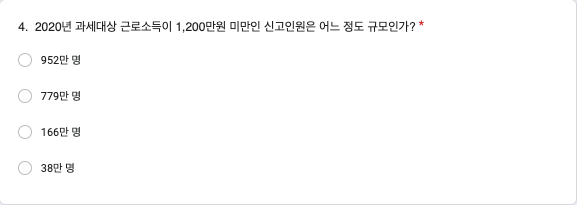
\includegraphics[width=0.75\linewidth]{./pics/Quiz230315_Q4}

\subsubsection{과세대상 근로소득 1,200만
원(집계표)}\label{uxacfcuxc138uxb300uxc0c1-uxadfcuxb85cuxc18cuxb4dd-1200uxb9cc-uxc6d0uxc9d1uxacc4uxd45c}

\begin{longtable}[]{@{}
  >{\raggedright\arraybackslash}p{(\columnwidth - 10\tabcolsep) * \real{0.1667}}
  >{\centering\arraybackslash}p{(\columnwidth - 10\tabcolsep) * \real{0.1528}}
  >{\centering\arraybackslash}p{(\columnwidth - 10\tabcolsep) * \real{0.1528}}
  >{\centering\arraybackslash}p{(\columnwidth - 10\tabcolsep) * \real{0.1528}}
  >{\centering\arraybackslash}p{(\columnwidth - 10\tabcolsep) * \real{0.1389}}
  >{\centering\arraybackslash}p{(\columnwidth - 10\tabcolsep) * \real{0.0833}}@{}}
\toprule\noalign{}
\begin{minipage}[b]{\linewidth}\raggedright
~
\end{minipage} & \begin{minipage}[b]{\linewidth}\centering
952만 명
\end{minipage} & \begin{minipage}[b]{\linewidth}\centering
779만 명
\end{minipage} & \begin{minipage}[b]{\linewidth}\centering
166만 명
\end{minipage} & \begin{minipage}[b]{\linewidth}\centering
38만 명
\end{minipage} & \begin{minipage}[b]{\linewidth}\centering
계
\end{minipage} \\
\midrule\noalign{}
\endhead
\bottomrule\noalign{}
\endlastfoot
\textbf{Red} & 158 & 71 & 39 & 9 & 277 \\
\textbf{Black} & 150 & 74 & 47 & 5 & 276 \\
\textbf{계} & 308 & 145 & 86 & 14 & 553 \\
\end{longtable}

\begin{longtable}[]{@{}
  >{\raggedleft\arraybackslash}p{(\columnwidth - 4\tabcolsep) * \real{0.2361}}
  >{\raggedleft\arraybackslash}p{(\columnwidth - 4\tabcolsep) * \real{0.0694}}
  >{\raggedleft\arraybackslash}p{(\columnwidth - 4\tabcolsep) * \real{0.1389}}@{}}
\caption{Pearson's Chi-squared test: \texttt{.}}\tabularnewline
\toprule\noalign{}
\begin{minipage}[b]{\linewidth}\raggedleft
Test statistic
\end{minipage} & \begin{minipage}[b]{\linewidth}\raggedleft
df
\end{minipage} & \begin{minipage}[b]{\linewidth}\raggedleft
P value
\end{minipage} \\
\midrule\noalign{}
\endfirsthead
\toprule\noalign{}
\begin{minipage}[b]{\linewidth}\raggedleft
Test statistic
\end{minipage} & \begin{minipage}[b]{\linewidth}\raggedleft
df
\end{minipage} & \begin{minipage}[b]{\linewidth}\raggedleft
P value
\end{minipage} \\
\midrule\noalign{}
\endhead
\bottomrule\noalign{}
\endlastfoot
2.155 & 3 & 0.5408 \\
\end{longtable}

Q4의 집계 결과가 Red, Black 간에 통계적으로 유의한 차이가 있는지
알아보기 위하여 카이제곱 테스트를 수행하였습니다.

그 결과 카이제곱 통계량은 2.155, 자유도는 3, p-value 는 0.5408이므로
Red, Black 간에 통계적으로 유의한 차이를 보이지 않습니다.

실제로 닮은 게 느껴집니까?

\subsubsection{과세대상 근로소득 1,200만
원(\%)}\label{uxacfcuxc138uxb300uxc0c1-uxadfcuxb85cuxc18cuxb4dd-1200uxb9cc-uxc6d0}

\begin{longtable}[]{@{}
  >{\centering\arraybackslash}p{(\columnwidth - 8\tabcolsep) * \real{0.1528}}
  >{\centering\arraybackslash}p{(\columnwidth - 8\tabcolsep) * \real{0.1528}}
  >{\centering\arraybackslash}p{(\columnwidth - 8\tabcolsep) * \real{0.1528}}
  >{\centering\arraybackslash}p{(\columnwidth - 8\tabcolsep) * \real{0.1389}}
  >{\centering\arraybackslash}p{(\columnwidth - 8\tabcolsep) * \real{0.1389}}@{}}
\toprule\noalign{}
\begin{minipage}[b]{\linewidth}\centering
952만 명
\end{minipage} & \begin{minipage}[b]{\linewidth}\centering
779만 명
\end{minipage} & \begin{minipage}[b]{\linewidth}\centering
166만 명
\end{minipage} & \begin{minipage}[b]{\linewidth}\centering
38만 명
\end{minipage} & \begin{minipage}[b]{\linewidth}\centering
계
\end{minipage} \\
\midrule\noalign{}
\endhead
\bottomrule\noalign{}
\endlastfoot
55.7 & 26.2 & 15.6 & 2.5 & 100.0 \\
\end{longtable}

정답률은 Red, Black 을 합하여 계산하는데, 55.7(\%) 입니다.

\subsection{Q5. 소득세
실효세율}\label{q5.-uxc18cuxb4dduxc138-uxc2e4uxd6a8uxc138uxc728}


\includegraphics[width=0.75\linewidth]{./pics/Quiz230315_Q5}

\subsubsection{소득세
실효세율(집계표)}\label{uxc18cuxb4dduxc138-uxc2e4uxd6a8uxc138uxc728uxc9d1uxacc4uxd45c}

\begin{longtable}[]{@{}
  >{\raggedright\arraybackslash}p{(\columnwidth - 10\tabcolsep) * \real{0.1667}}
  >{\raggedleft\arraybackslash}p{(\columnwidth - 10\tabcolsep) * \real{0.0972}}
  >{\raggedleft\arraybackslash}p{(\columnwidth - 10\tabcolsep) * \real{0.1111}}
  >{\raggedleft\arraybackslash}p{(\columnwidth - 10\tabcolsep) * \real{0.1111}}
  >{\raggedleft\arraybackslash}p{(\columnwidth - 10\tabcolsep) * \real{0.0972}}
  >{\centering\arraybackslash}p{(\columnwidth - 10\tabcolsep) * \real{0.0972}}@{}}
\toprule\noalign{}
\begin{minipage}[b]{\linewidth}\raggedright
~
\end{minipage} & \begin{minipage}[b]{\linewidth}\raggedleft
0.2\%
\end{minipage} & \begin{minipage}[b]{\linewidth}\raggedleft
15.1\%
\end{minipage} & \begin{minipage}[b]{\linewidth}\raggedleft
37.4\%
\end{minipage} & \begin{minipage}[b]{\linewidth}\raggedleft
5.9\%
\end{minipage} & \begin{minipage}[b]{\linewidth}\centering
계
\end{minipage} \\
\midrule\noalign{}
\endhead
\bottomrule\noalign{}
\endlastfoot
\textbf{Red} & 2 & 58 & 19 & 198 & 277 \\
\textbf{Black} & 8 & 48 & 16 & 204 & 276 \\
\textbf{계} & 10 & 106 & 35 & 402 & 553 \\
\end{longtable}

\begin{longtable}[]{@{}
  >{\raggedleft\arraybackslash}p{(\columnwidth - 4\tabcolsep) * \real{0.2361}}
  >{\raggedleft\arraybackslash}p{(\columnwidth - 4\tabcolsep) * \real{0.0694}}
  >{\raggedleft\arraybackslash}p{(\columnwidth - 4\tabcolsep) * \real{0.1389}}@{}}
\caption{Pearson's Chi-squared test: \texttt{.}}\tabularnewline
\toprule\noalign{}
\begin{minipage}[b]{\linewidth}\raggedleft
Test statistic
\end{minipage} & \begin{minipage}[b]{\linewidth}\raggedleft
df
\end{minipage} & \begin{minipage}[b]{\linewidth}\raggedleft
P value
\end{minipage} \\
\midrule\noalign{}
\endfirsthead
\toprule\noalign{}
\begin{minipage}[b]{\linewidth}\raggedleft
Test statistic
\end{minipage} & \begin{minipage}[b]{\linewidth}\raggedleft
df
\end{minipage} & \begin{minipage}[b]{\linewidth}\raggedleft
P value
\end{minipage} \\
\midrule\noalign{}
\endhead
\bottomrule\noalign{}
\endlastfoot
4.888 & 3 & 0.1802 \\
\end{longtable}

Q5의 집계 결과가 Red, Black 간에 통계적으로 유의한 차이가 있는지
알아보기 위하여 카이제곱 테스트를 수행하였습니다.

그 결과 카이제곱 통계량은 4.888, 자유도는 3, p-value 는 0.1802이므로
Red, Black 간에 통계적으로 유의한 차이를 보이지 않습니다.

실제로 닮은 게 느껴집니까?

\subsubsection{소득세
실효세율(\%)}\label{uxc18cuxb4dduxc138-uxc2e4uxd6a8uxc138uxc728}

\begin{longtable}[]{@{}
  >{\raggedleft\arraybackslash}p{(\columnwidth - 8\tabcolsep) * \real{0.0972}}
  >{\raggedleft\arraybackslash}p{(\columnwidth - 8\tabcolsep) * \real{0.1111}}
  >{\raggedleft\arraybackslash}p{(\columnwidth - 8\tabcolsep) * \real{0.1111}}
  >{\raggedleft\arraybackslash}p{(\columnwidth - 8\tabcolsep) * \real{0.0972}}
  >{\centering\arraybackslash}p{(\columnwidth - 8\tabcolsep) * \real{0.1111}}@{}}
\toprule\noalign{}
\begin{minipage}[b]{\linewidth}\raggedleft
0.2\%
\end{minipage} & \begin{minipage}[b]{\linewidth}\raggedleft
15.1\%
\end{minipage} & \begin{minipage}[b]{\linewidth}\raggedleft
37.4\%
\end{minipage} & \begin{minipage}[b]{\linewidth}\raggedleft
5.9\%
\end{minipage} & \begin{minipage}[b]{\linewidth}\centering
계
\end{minipage} \\
\midrule\noalign{}
\endhead
\bottomrule\noalign{}
\endlastfoot
1.8 & 19.2 & 6.3 & 72.7 & 100.0 \\
\end{longtable}

정답률은 Red, Black 을 합하여 계산하는데, 72.7(\%) 입니다.

\subsection{Q6. 기업규모별 과세
현황}\label{q6.-uxae30uxc5c5uxaddcuxbaa8uxbcc4-uxacfcuxc138-uxd604uxd669}

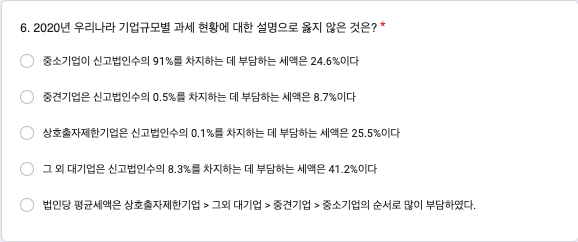
\includegraphics[width=0.75\linewidth]{./pics/Quiz230315_Q6}

\subsubsection{기업규모별 과세
현황(집계표)}\label{uxae30uxc5c5uxaddcuxbaa8uxbcc4-uxacfcuxc138-uxd604uxd669uxc9d1uxacc4uxd45c}

\begin{longtable}[]{@{}
  >{\raggedright\arraybackslash}p{(\columnwidth - 12\tabcolsep) * \real{0.0678}}
  >{\centering\arraybackslash}p{(\columnwidth - 12\tabcolsep) * \real{0.1808}}
  >{\centering\arraybackslash}p{(\columnwidth - 12\tabcolsep) * \real{0.1864}}
  >{\centering\arraybackslash}p{(\columnwidth - 12\tabcolsep) * \real{0.1751}}
  >{\centering\arraybackslash}p{(\columnwidth - 12\tabcolsep) * \real{0.1695}}
  >{\centering\arraybackslash}p{(\columnwidth - 12\tabcolsep) * \real{0.1864}}
  >{\centering\arraybackslash}p{(\columnwidth - 12\tabcolsep) * \real{0.0339}}@{}}
\toprule\noalign{}
\begin{minipage}[b]{\linewidth}\raggedright
~
\end{minipage} & \begin{minipage}[b]{\linewidth}\centering
중소기업이 신고법인수의 91\%를 차지하는 데 부담하는 세액은 24.6\%이다
\end{minipage} & \begin{minipage}[b]{\linewidth}\centering
중견기업은 신고법인수의 0.5\%를 차지하는 데 부담하는 세액은 8.7\%이다
\end{minipage} & \begin{minipage}[b]{\linewidth}\centering
상호출자제한기업은 신고법인수의 0.1\%를 차지하는 데 부담하는 세액은
25.5\%이다
\end{minipage} & \begin{minipage}[b]{\linewidth}\centering
그 외 대기업은 신고법인수의 8.3\%를 차지하는 데 부담하는 세액은
41.2\%이다
\end{minipage} & \begin{minipage}[b]{\linewidth}\centering
법인당 평균세액은 상호출자제한기업 \textgreater{} 그외 대기업
\textgreater{} 중견기업 \textgreater{} 중소기업의 순서로 많이
부담하였다.
\end{minipage} & \begin{minipage}[b]{\linewidth}\centering
계
\end{minipage} \\
\midrule\noalign{}
\endhead
\bottomrule\noalign{}
\endlastfoot
\textbf{Red} & 14 & 37 & 38 & 50 & 138 & 277 \\
\textbf{Black} & 18 & 33 & 21 & 61 & 143 & 276 \\
\textbf{계} & 32 & 70 & 59 & 111 & 281 & 553 \\
\end{longtable}

\begin{longtable}[]{@{}
  >{\raggedleft\arraybackslash}p{(\columnwidth - 4\tabcolsep) * \real{0.2361}}
  >{\raggedleft\arraybackslash}p{(\columnwidth - 4\tabcolsep) * \real{0.0694}}
  >{\raggedleft\arraybackslash}p{(\columnwidth - 4\tabcolsep) * \real{0.1389}}@{}}
\caption{Pearson's Chi-squared test: \texttt{.}}\tabularnewline
\toprule\noalign{}
\begin{minipage}[b]{\linewidth}\raggedleft
Test statistic
\end{minipage} & \begin{minipage}[b]{\linewidth}\raggedleft
df
\end{minipage} & \begin{minipage}[b]{\linewidth}\raggedleft
P value
\end{minipage} \\
\midrule\noalign{}
\endfirsthead
\toprule\noalign{}
\begin{minipage}[b]{\linewidth}\raggedleft
Test statistic
\end{minipage} & \begin{minipage}[b]{\linewidth}\raggedleft
df
\end{minipage} & \begin{minipage}[b]{\linewidth}\raggedleft
P value
\end{minipage} \\
\midrule\noalign{}
\endhead
\bottomrule\noalign{}
\endlastfoot
6.804 & 4 & 0.1466 \\
\end{longtable}

Q6의 집계 결과가 Red, Black 간에 통계적으로 유의한 차이가 있는지
알아보기 위하여 카이제곱 테스트를 수행하였습니다.

그 결과 카이제곱 통계량은 6.804, 자유도는 4, p-value 는 0.1466이므로
Red, Black 간에 통계적으로 유의한 차이를 보이지 않습니다.

실제로 닮은 게 느껴집니까?

\subsubsection{기업규모별 과세
현황(\%)}\label{uxae30uxc5c5uxaddcuxbaa8uxbcc4-uxacfcuxc138-uxd604uxd669}

\begin{longtable}[]{@{}
  >{\centering\arraybackslash}p{(\columnwidth - 10\tabcolsep) * \real{0.1916}}
  >{\centering\arraybackslash}p{(\columnwidth - 10\tabcolsep) * \real{0.1976}}
  >{\centering\arraybackslash}p{(\columnwidth - 10\tabcolsep) * \real{0.1856}}
  >{\centering\arraybackslash}p{(\columnwidth - 10\tabcolsep) * \real{0.1796}}
  >{\centering\arraybackslash}p{(\columnwidth - 10\tabcolsep) * \real{0.1976}}
  >{\centering\arraybackslash}p{(\columnwidth - 10\tabcolsep) * \real{0.0479}}@{}}
\toprule\noalign{}
\begin{minipage}[b]{\linewidth}\centering
중소기업이 신고법인수의 91\%를 차지하는 데 부담하는 세액은 24.6\%이다
\end{minipage} & \begin{minipage}[b]{\linewidth}\centering
중견기업은 신고법인수의 0.5\%를 차지하는 데 부담하는 세액은 8.7\%이다
\end{minipage} & \begin{minipage}[b]{\linewidth}\centering
상호출자제한기업은 신고법인수의 0.1\%를 차지하는 데 부담하는 세액은
25.5\%이다
\end{minipage} & \begin{minipage}[b]{\linewidth}\centering
그 외 대기업은 신고법인수의 8.3\%를 차지하는 데 부담하는 세액은
41.2\%이다
\end{minipage} & \begin{minipage}[b]{\linewidth}\centering
법인당 평균세액은 상호출자제한기업 \textgreater{} 그외 대기업
\textgreater{} 중견기업 \textgreater{} 중소기업의 순서로 많이
부담하였다.
\end{minipage} & \begin{minipage}[b]{\linewidth}\centering
계
\end{minipage} \\
\midrule\noalign{}
\endhead
\bottomrule\noalign{}
\endlastfoot
5.8 & 12.7 & 10.7 & 20.1 & 50.8 & 100.0 \\
\end{longtable}

정답률은 Red, Black 을 합하여 계산하는데, 50.8(\%) 입니다.

\subsection{Q7. 국민부담률 적정 수준 : 아일랜드와 OECD
평균}\label{q7.-uxad6duxbbfcuxbd80uxb2f4uxb960-uxc801uxc815-uxc218uxc900-uxc544uxc77cuxb79cuxb4dcuxc640-oecd-uxd3c9uxade0}

질문 내용에 의도하는 바를 담으면 어떨까요?

OECD 국가 중 국민부담률이 매우 낮은 편인 아일랜드의 사례를 들어서
감세정책이 가져온 긍정적인 효과에 대해서 설명하고 우리나라의 바람직한
조정 방향은 무엇이냐고 묻는 것을 Red, 감세 정책이 가져온 부정적인 효과에
대해서 설명하고 우리나라의 바람직한 조정 방향은 무엇이냐고 묻는 것을
Black 에 배치했을 때, 설명이 응답에 영향을 미치지 않으면 Red 와 Black에
차이가 없어야 할텐데 집계결과는 어떻게 나오고 있나요?

분명히 영향을 미치고 있는 것으로 보입니다.

통계적으로 매우 유의한 차이가 관찰되고 있습니다.

감세정책의 효과가 긍정적이라고 설명한 Red 에서는 낮춰야 한다는 응답이,
감세정책의 효과가 부정적이라고 설명한 Black 에서는 높여야 한다는 응답이
높게 나온 것을 볼 수 있고, 따라서 p-value 가 엄청나게 작은 값을 보여주고
있습니다.

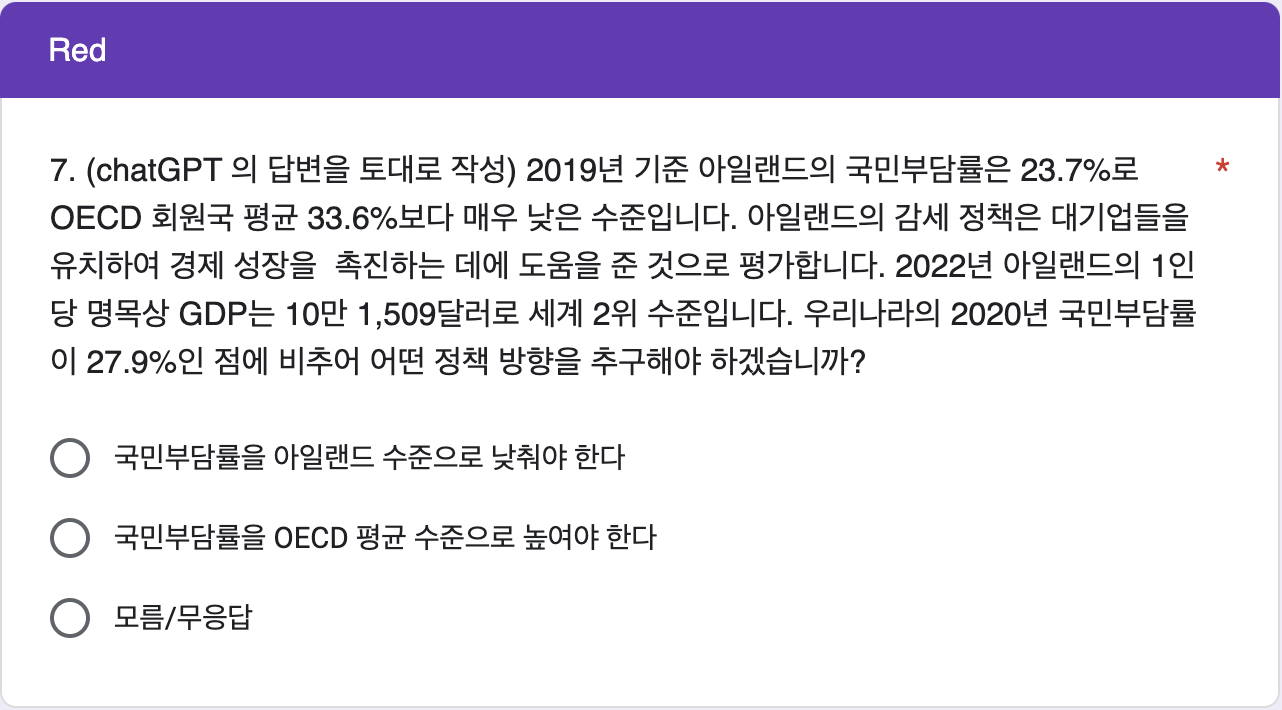
\includegraphics[width=0.67\linewidth]{./pics/Quiz240315_Q7_Red}

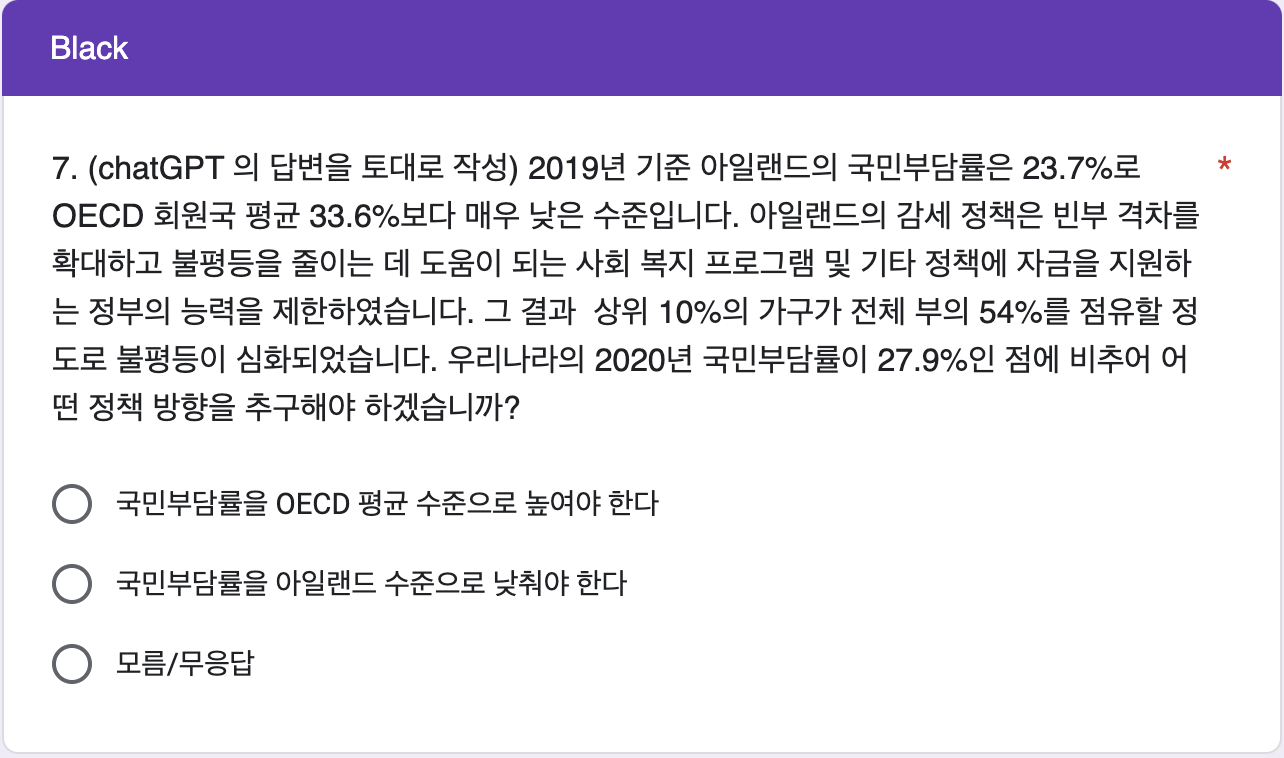
\includegraphics[width=0.67\linewidth]{./pics/Quiz240315_Q7_Black}

\subsubsection{집계표}\label{uxc9d1uxacc4uxd45c}

\begin{longtable}[]{@{}
  >{\raggedright\arraybackslash}p{(\columnwidth - 8\tabcolsep) * \real{0.3766}}
  >{\centering\arraybackslash}p{(\columnwidth - 8\tabcolsep) * \real{0.1818}}
  >{\centering\arraybackslash}p{(\columnwidth - 8\tabcolsep) * \real{0.1818}}
  >{\centering\arraybackslash}p{(\columnwidth - 8\tabcolsep) * \real{0.1818}}
  >{\centering\arraybackslash}p{(\columnwidth - 8\tabcolsep) * \real{0.0779}}@{}}
\toprule\noalign{}
\begin{minipage}[b]{\linewidth}\raggedright
~
\end{minipage} & \begin{minipage}[b]{\linewidth}\centering
낮춰야 한다
\end{minipage} & \begin{minipage}[b]{\linewidth}\centering
높여야 한다
\end{minipage} & \begin{minipage}[b]{\linewidth}\centering
모름/무응답
\end{minipage} & \begin{minipage}[b]{\linewidth}\centering
계
\end{minipage} \\
\midrule\noalign{}
\endhead
\bottomrule\noalign{}
\endlastfoot
\textbf{Red(감세의 긍정적효과 설명)} & 90 & 120 & 67 & 277 \\
\textbf{Black(감세의 부정적 효과 설명)} & 46 & 168 & 62 & 276 \\
\textbf{계} & 136 & 288 & 129 & 553 \\
\end{longtable}

\begin{longtable}[]{@{}
  >{\raggedleft\arraybackslash}p{(\columnwidth - 4\tabcolsep) * \real{0.2361}}
  >{\raggedleft\arraybackslash}p{(\columnwidth - 4\tabcolsep) * \real{0.0694}}
  >{\raggedleft\arraybackslash}p{(\columnwidth - 4\tabcolsep) * \real{0.2500}}@{}}
\caption{Pearson's Chi-squared test: \texttt{.}}\tabularnewline
\toprule\noalign{}
\begin{minipage}[b]{\linewidth}\raggedleft
Test statistic
\end{minipage} & \begin{minipage}[b]{\linewidth}\raggedleft
df
\end{minipage} & \begin{minipage}[b]{\linewidth}\raggedleft
P value
\end{minipage} \\
\midrule\noalign{}
\endfirsthead
\toprule\noalign{}
\begin{minipage}[b]{\linewidth}\raggedleft
Test statistic
\end{minipage} & \begin{minipage}[b]{\linewidth}\raggedleft
df
\end{minipage} & \begin{minipage}[b]{\linewidth}\raggedleft
P value
\end{minipage} \\
\midrule\noalign{}
\endhead
\bottomrule\noalign{}
\endlastfoot
22.43 & 2 & 1.349e-05 * * * \\
\end{longtable}

Q7의 Red에는 아일랜드의 사례에서 감세 정책의 긍정적 측면을 설명한 후
우리나라 조세 정책의 방향에 대하여 물었을 때, 277명이 응답한 가운데
90명이 우리나라의 국민부담률을 아일랜드 수준으로 ``낮춰야 한다''는
반응을 보이고, 120명이 OECD평균 수준으로 ``높여야 한다''는 반응을
보입니다.

Black은 같은 아일랜드의 사례에서 감세 정책의 부정적 측면을 설명한 후
우리나라 조세 정책의 방향에 대하여 물었을 떄, 276명이 응답한 가운데
46명이 우리나라의 국민부담률을 아일랜드 수준으로 ``낮춰야 한다''는
반응을 보이고, 168명이 OECD 평균 수준으로 ``높여야 한다''는 반응을
보입니다.

그리고 ``모름/무응답''에 답한 인원은 Red에 67명, Black 에 62명이
응답하였습니다.

우연일까요?

모름/무응답에 있어서는 Red, Black이 몹시 닮았습니다.

카이제곱 테스트는 이와 같은 상황에서 감세정책의 긍정적 측면을 부각시킨
경우와 부정적 측면을 부각시킨 경우에 그 차이가 통계적으로 매우, 매우,
\ldots{} 유의하다는 것을 보여 줍니다.

카이제곱 통계량은 22.427, 자유도는 2, p-value 는 1.3e-05으로 감세정책의
어떤 측면을 설명하느냐에 따라 반응이 다르게 나온다는 것을 보여줍니다.

여기서 질문 내용에 의도하는 바를 담더라도 응답에 영향을 끼치지 않는다고
가정합니다.

랜덤화의 효과로 Red, Black 의 응답은 닮게 마련입니다.

즉, 통계적으로 유의한 차이를 보이지 않게 됩니다.

그러나 실제로 관찰된 카이제곱 통계값의 P-value 는 0.05보다 매우 작은
값입니다.

따라서, 질문 내용에 의도하는 바를 담더라도 영향을 끼치지 않는다는 가정은
잘못된 것이죠.

이러한 논증 방식을 귀류법이라고 합니다.

\subsubsection{\% 비교}\label{uxbe44uxad50}

\begin{longtable}[]{@{}
  >{\raggedright\arraybackslash}p{(\columnwidth - 8\tabcolsep) * \real{0.3671}}
  >{\centering\arraybackslash}p{(\columnwidth - 8\tabcolsep) * \real{0.1772}}
  >{\centering\arraybackslash}p{(\columnwidth - 8\tabcolsep) * \real{0.1772}}
  >{\centering\arraybackslash}p{(\columnwidth - 8\tabcolsep) * \real{0.1772}}
  >{\centering\arraybackslash}p{(\columnwidth - 8\tabcolsep) * \real{0.1013}}@{}}
\toprule\noalign{}
\begin{minipage}[b]{\linewidth}\raggedright
~
\end{minipage} & \begin{minipage}[b]{\linewidth}\centering
낮춰야 한다
\end{minipage} & \begin{minipage}[b]{\linewidth}\centering
높여야 한다
\end{minipage} & \begin{minipage}[b]{\linewidth}\centering
모름/무응답
\end{minipage} & \begin{minipage}[b]{\linewidth}\centering
계
\end{minipage} \\
\midrule\noalign{}
\endhead
\bottomrule\noalign{}
\endlastfoot
\textbf{Red(감세의 긍정적효과 설명)} & 32.5 & 43.3 & 24.2 & 100.0 \\
\textbf{Black(감세의 부정적 효과 설명)} & 16.7 & 60.9 & 22.5 & 100.0 \\
\end{longtable}

감세정책의 긍정적 측면을 설명한 Red에서 우리나라의 국민부담률을 ``낮춰야
한다''고 응답하는사람들의 백분율, 32.5(\%)은 ``높여야 한다''고 응답하는
사람들의 백분율, 43.3(\%) 보다 높습니다.

반면 감세정책의 부정적 측면을 설명한 Black에서 우리나라의 국민 부담률을
``낮춰야 한다''고 응답하는 사람들의 백분율, 16.7(\%)은 ``높여야 한다''고
응답하는 사람들의 백분율, 60.9(\%) 보다 훨씬 적습니다.

어느 정책의 긍정적 측면을 설명하느냐, 부정적 측면을 설명하느냐에 따라
반응이 달라진다는 것을 잘 알 수 있습니다.

Red 와 Black 이 워낙 차이가 나지만 전체적으로 어느 정도가 우리나라의
국민부담률을 ``낮춰야 한다''하고 어느 정도가 ``높여야 한다''고
응답하였는지 합쳐 보겠습니다.

\subsubsection{\% 합계}\label{uxd569uxacc4}

\begin{longtable}[]{@{}
  >{\centering\arraybackslash}p{(\columnwidth - 6\tabcolsep) * \real{0.1944}}
  >{\centering\arraybackslash}p{(\columnwidth - 6\tabcolsep) * \real{0.1944}}
  >{\centering\arraybackslash}p{(\columnwidth - 6\tabcolsep) * \real{0.1944}}
  >{\centering\arraybackslash}p{(\columnwidth - 6\tabcolsep) * \real{0.1111}}@{}}
\toprule\noalign{}
\begin{minipage}[b]{\linewidth}\centering
낮춰야 한다
\end{minipage} & \begin{minipage}[b]{\linewidth}\centering
높여야 한다
\end{minipage} & \begin{minipage}[b]{\linewidth}\centering
모름/무응답
\end{minipage} & \begin{minipage}[b]{\linewidth}\centering
계
\end{minipage} \\
\midrule\noalign{}
\endhead
\bottomrule\noalign{}
\endlastfoot
24.6 & 52.1 & 23.3 & 100.0 \\
\end{longtable}

우리나라의 국민부담률을 ``낮춰야 한다''고 응답한 백분율은 Red, Black
합쳐서 24.6(\%)(으)로 우리나라의 국민부담률을 '높여야한다''고 응답한
백분율, 52.1(\%) 보다 상당히 적습니다.

다만, 모름/무응답이 23.3(\%)로 적지 않습니다.

\subsubsection{Mosaic Plot}\label{mosaic-plot}


\includegraphics{quiz250317_Report_v6_files/figure-latex/mosaic plot-1.pdf}

Mosaic Plot 은 이 집계결과를 시각적으로 잘 보여줍니다.

감세정책의 긍정적 측면을 설명한 Red 에서 우리나라의 국민부담률을
``낮춰야 한다''고 응답한 백분율이 높고, 감세정책의 부정적 측면을 설명한
Black 에서 우리나라의 국민부담률을 ``높여야 한다''고 응답한 백분율이
월등히 높은 것을 시각적으로 알 수 있습니다.

\subsection{마감 시간으로부터 제출 시간의
분포}\label{uxb9c8uxac10-uxc2dcuxac04uxc73cuxb85cuxbd80uxd130-uxc81cuxcd9c-uxc2dcuxac04uxc758-uxbd84uxd3ec}

\subsubsection{분포표}\label{uxbd84uxd3ecuxd45c}

\begin{longtable}[]{@{}
  >{\raggedright\arraybackslash}p{(\columnwidth - 30\tabcolsep) * \real{0.0863}}
  >{\raggedleft\arraybackslash}p{(\columnwidth - 30\tabcolsep) * \real{0.0576}}
  >{\raggedleft\arraybackslash}p{(\columnwidth - 30\tabcolsep) * \real{0.0576}}
  >{\raggedleft\arraybackslash}p{(\columnwidth - 30\tabcolsep) * \real{0.0576}}
  >{\raggedleft\arraybackslash}p{(\columnwidth - 30\tabcolsep) * \real{0.0576}}
  >{\raggedleft\arraybackslash}p{(\columnwidth - 30\tabcolsep) * \real{0.0576}}
  >{\raggedleft\arraybackslash}p{(\columnwidth - 30\tabcolsep) * \real{0.0576}}
  >{\raggedleft\arraybackslash}p{(\columnwidth - 30\tabcolsep) * \real{0.0576}}
  >{\raggedleft\arraybackslash}p{(\columnwidth - 30\tabcolsep) * \real{0.0576}}
  >{\raggedleft\arraybackslash}p{(\columnwidth - 30\tabcolsep) * \real{0.0576}}
  >{\raggedleft\arraybackslash}p{(\columnwidth - 30\tabcolsep) * \real{0.0647}}
  >{\raggedleft\arraybackslash}p{(\columnwidth - 30\tabcolsep) * \real{0.0719}}
  >{\raggedleft\arraybackslash}p{(\columnwidth - 30\tabcolsep) * \real{0.0719}}
  >{\raggedleft\arraybackslash}p{(\columnwidth - 30\tabcolsep) * \real{0.0719}}
  >{\raggedleft\arraybackslash}p{(\columnwidth - 30\tabcolsep) * \real{0.0719}}
  >{\centering\arraybackslash}p{(\columnwidth - 30\tabcolsep) * \real{0.0432}}@{}}
\caption{일 단위}\tabularnewline
\toprule\noalign{}
\begin{minipage}[b]{\linewidth}\raggedright
~
\end{minipage} & \begin{minipage}[b]{\linewidth}\raggedleft
{[}0,1{]}
\end{minipage} & \begin{minipage}[b]{\linewidth}\raggedleft
(1,2{]}
\end{minipage} & \begin{minipage}[b]{\linewidth}\raggedleft
(2,3{]}
\end{minipage} & \begin{minipage}[b]{\linewidth}\raggedleft
(3,4{]}
\end{minipage} & \begin{minipage}[b]{\linewidth}\raggedleft
(4,5{]}
\end{minipage} & \begin{minipage}[b]{\linewidth}\raggedleft
(5,6{]}
\end{minipage} & \begin{minipage}[b]{\linewidth}\raggedleft
(6,7{]}
\end{minipage} & \begin{minipage}[b]{\linewidth}\raggedleft
(7,8{]}
\end{minipage} & \begin{minipage}[b]{\linewidth}\raggedleft
(8,9{]}
\end{minipage} & \begin{minipage}[b]{\linewidth}\raggedleft
(9,10{]}
\end{minipage} & \begin{minipage}[b]{\linewidth}\raggedleft
(10,11{]}
\end{minipage} & \begin{minipage}[b]{\linewidth}\raggedleft
(11,12{]}
\end{minipage} & \begin{minipage}[b]{\linewidth}\raggedleft
(12,13{]}
\end{minipage} & \begin{minipage}[b]{\linewidth}\raggedleft
(13,14{]}
\end{minipage} & \begin{minipage}[b]{\linewidth}\centering
계
\end{minipage} \\
\midrule\noalign{}
\endfirsthead
\toprule\noalign{}
\begin{minipage}[b]{\linewidth}\raggedright
~
\end{minipage} & \begin{minipage}[b]{\linewidth}\raggedleft
{[}0,1{]}
\end{minipage} & \begin{minipage}[b]{\linewidth}\raggedleft
(1,2{]}
\end{minipage} & \begin{minipage}[b]{\linewidth}\raggedleft
(2,3{]}
\end{minipage} & \begin{minipage}[b]{\linewidth}\raggedleft
(3,4{]}
\end{minipage} & \begin{minipage}[b]{\linewidth}\raggedleft
(4,5{]}
\end{minipage} & \begin{minipage}[b]{\linewidth}\raggedleft
(5,6{]}
\end{minipage} & \begin{minipage}[b]{\linewidth}\raggedleft
(6,7{]}
\end{minipage} & \begin{minipage}[b]{\linewidth}\raggedleft
(7,8{]}
\end{minipage} & \begin{minipage}[b]{\linewidth}\raggedleft
(8,9{]}
\end{minipage} & \begin{minipage}[b]{\linewidth}\raggedleft
(9,10{]}
\end{minipage} & \begin{minipage}[b]{\linewidth}\raggedleft
(10,11{]}
\end{minipage} & \begin{minipage}[b]{\linewidth}\raggedleft
(11,12{]}
\end{minipage} & \begin{minipage}[b]{\linewidth}\raggedleft
(12,13{]}
\end{minipage} & \begin{minipage}[b]{\linewidth}\raggedleft
(13,14{]}
\end{minipage} & \begin{minipage}[b]{\linewidth}\centering
계
\end{minipage} \\
\midrule\noalign{}
\endhead
\bottomrule\noalign{}
\endlastfoot
\textbf{Red} & 71 & 12 & 6 & 8 & 4 & 6 & 16 & 48 & 20 & 14 & 18 & 17 &
16 & 21 & 277 \\
\textbf{Black} & 64 & 14 & 3 & 6 & 10 & 4 & 4 & 47 & 30 & 18 & 12 & 17 &
22 & 25 & 276 \\
\textbf{계} & 135 & 26 & 9 & 14 & 14 & 10 & 20 & 95 & 50 & 32 & 30 & 34
& 38 & 46 & 553 \\
\end{longtable}

분포표로부터 두 가지 문제를 살펴보겠습니다.

첫째, 날마다 고르게 제출하는가?

둘째, Red, Black 간에 통계적으로 유의한 차이가 있는가?

각 문제를 살펴보기 위해서는 분포표의 일부분을 대상으로 카이제곱 테스트를
수행합니다.

\subsubsection{날마다 고르게
제출하는가?}\label{uxb0a0uxb9c8uxb2e4-uxace0uxb974uxac8c-uxc81cuxcd9cuxd558uxb294uxac00}

\begin{longtable}[]{@{}
  >{\raggedleft\arraybackslash}p{(\columnwidth - 26\tabcolsep) * \real{0.0661}}
  >{\raggedleft\arraybackslash}p{(\columnwidth - 26\tabcolsep) * \real{0.0661}}
  >{\raggedleft\arraybackslash}p{(\columnwidth - 26\tabcolsep) * \real{0.0661}}
  >{\raggedleft\arraybackslash}p{(\columnwidth - 26\tabcolsep) * \real{0.0661}}
  >{\raggedleft\arraybackslash}p{(\columnwidth - 26\tabcolsep) * \real{0.0661}}
  >{\raggedleft\arraybackslash}p{(\columnwidth - 26\tabcolsep) * \real{0.0661}}
  >{\raggedleft\arraybackslash}p{(\columnwidth - 26\tabcolsep) * \real{0.0661}}
  >{\raggedleft\arraybackslash}p{(\columnwidth - 26\tabcolsep) * \real{0.0661}}
  >{\raggedleft\arraybackslash}p{(\columnwidth - 26\tabcolsep) * \real{0.0661}}
  >{\raggedleft\arraybackslash}p{(\columnwidth - 26\tabcolsep) * \real{0.0744}}
  >{\raggedleft\arraybackslash}p{(\columnwidth - 26\tabcolsep) * \real{0.0826}}
  >{\raggedleft\arraybackslash}p{(\columnwidth - 26\tabcolsep) * \real{0.0826}}
  >{\raggedleft\arraybackslash}p{(\columnwidth - 26\tabcolsep) * \real{0.0826}}
  >{\raggedleft\arraybackslash}p{(\columnwidth - 26\tabcolsep) * \real{0.0826}}@{}}
\toprule\noalign{}
\begin{minipage}[b]{\linewidth}\raggedleft
{[}0,1{]}
\end{minipage} & \begin{minipage}[b]{\linewidth}\raggedleft
(1,2{]}
\end{minipage} & \begin{minipage}[b]{\linewidth}\raggedleft
(2,3{]}
\end{minipage} & \begin{minipage}[b]{\linewidth}\raggedleft
(3,4{]}
\end{minipage} & \begin{minipage}[b]{\linewidth}\raggedleft
(4,5{]}
\end{minipage} & \begin{minipage}[b]{\linewidth}\raggedleft
(5,6{]}
\end{minipage} & \begin{minipage}[b]{\linewidth}\raggedleft
(6,7{]}
\end{minipage} & \begin{minipage}[b]{\linewidth}\raggedleft
(7,8{]}
\end{minipage} & \begin{minipage}[b]{\linewidth}\raggedleft
(8,9{]}
\end{minipage} & \begin{minipage}[b]{\linewidth}\raggedleft
(9,10{]}
\end{minipage} & \begin{minipage}[b]{\linewidth}\raggedleft
(10,11{]}
\end{minipage} & \begin{minipage}[b]{\linewidth}\raggedleft
(11,12{]}
\end{minipage} & \begin{minipage}[b]{\linewidth}\raggedleft
(12,13{]}
\end{minipage} & \begin{minipage}[b]{\linewidth}\raggedleft
(13,14{]}
\end{minipage} \\
\midrule\noalign{}
\endhead
\bottomrule\noalign{}
\endlastfoot
135 & 26 & 9 & 14 & 14 & 10 & 20 & 95 & 50 & 32 & 30 & 34 & 38 & 46 \\
\end{longtable}

\begin{longtable}[]{@{}
  >{\raggedleft\arraybackslash}p{(\columnwidth - 4\tabcolsep) * \real{0.2361}}
  >{\raggedleft\arraybackslash}p{(\columnwidth - 4\tabcolsep) * \real{0.0694}}
  >{\raggedleft\arraybackslash}p{(\columnwidth - 4\tabcolsep) * \real{0.2500}}@{}}
\caption{Chi-squared test for given probabilities:
\texttt{.}}\tabularnewline
\toprule\noalign{}
\begin{minipage}[b]{\linewidth}\raggedleft
Test statistic
\end{minipage} & \begin{minipage}[b]{\linewidth}\raggedleft
df
\end{minipage} & \begin{minipage}[b]{\linewidth}\raggedleft
P value
\end{minipage} \\
\midrule\noalign{}
\endfirsthead
\toprule\noalign{}
\begin{minipage}[b]{\linewidth}\raggedleft
Test statistic
\end{minipage} & \begin{minipage}[b]{\linewidth}\raggedleft
df
\end{minipage} & \begin{minipage}[b]{\linewidth}\raggedleft
P value
\end{minipage} \\
\midrule\noalign{}
\endhead
\bottomrule\noalign{}
\endlastfoot
410 & 13 & 1.714e-79 * * * \\
\end{longtable}

날마다 고르게 제출하는지 알아 보았습니다.

분포표의 ``계''행에서 '계'열을 제외하고 카이제곱테스트를 수행합니다.

분포표 만으로도 쉽게 파악할 수 있지만 카이제곱테스트가 명확히 해 줍니다.

카이제곱 통계량은 410.01, 자유도는 13.00, p-value 는 1.7e-79 이므로 결코
고르게 제출한다고 말할 수 없겠습니다.

막대그래프로 살펴 보겠습니다.

\subsubsection{막대그래프}\label{uxb9c9uxb300uxadf8uxb798uxd504}

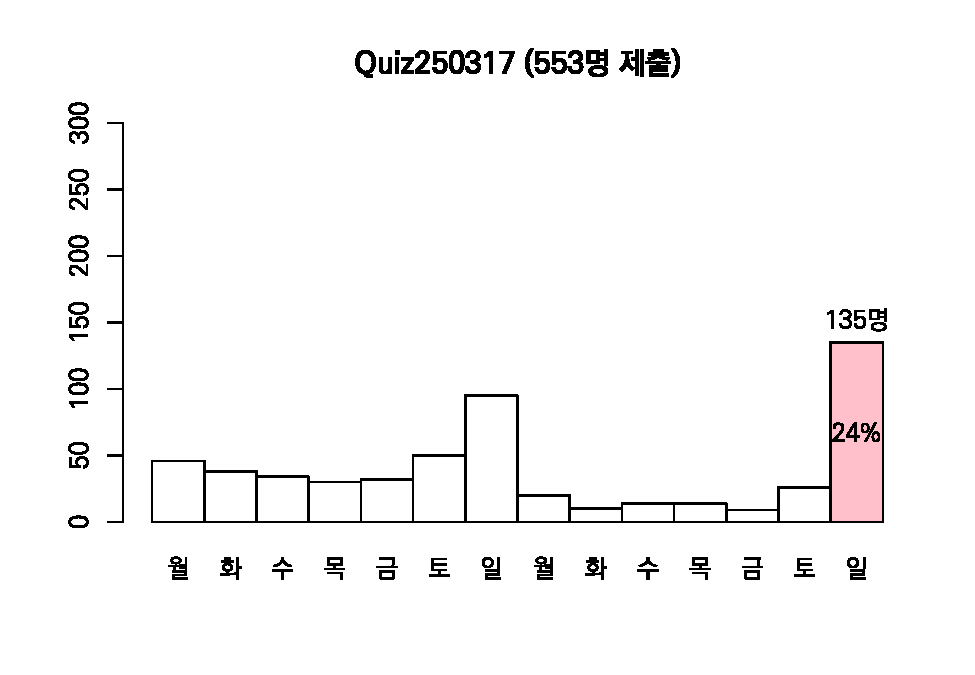
\includegraphics{quiz250317_Report_v6_files/figure-latex/unnamed-chunk-13-1.pdf}

막대그래프는 총 제출인원 553(명) 중에 135(명), 24(\%)가 마감일에 몰리는
것을 명확히 보여주고 있습니다.

\subsubsection{Red, Black 간에
닮았는가?}\label{red-black-uxac04uxc5d0-uxb2eeuxc558uxb294uxac00}

\begin{longtable}[]{@{}
  >{\raggedright\arraybackslash}p{(\columnwidth - 28\tabcolsep) * \real{0.0902}}
  >{\raggedleft\arraybackslash}p{(\columnwidth - 28\tabcolsep) * \real{0.0602}}
  >{\raggedleft\arraybackslash}p{(\columnwidth - 28\tabcolsep) * \real{0.0602}}
  >{\raggedleft\arraybackslash}p{(\columnwidth - 28\tabcolsep) * \real{0.0602}}
  >{\raggedleft\arraybackslash}p{(\columnwidth - 28\tabcolsep) * \real{0.0602}}
  >{\raggedleft\arraybackslash}p{(\columnwidth - 28\tabcolsep) * \real{0.0602}}
  >{\raggedleft\arraybackslash}p{(\columnwidth - 28\tabcolsep) * \real{0.0602}}
  >{\raggedleft\arraybackslash}p{(\columnwidth - 28\tabcolsep) * \real{0.0602}}
  >{\raggedleft\arraybackslash}p{(\columnwidth - 28\tabcolsep) * \real{0.0602}}
  >{\raggedleft\arraybackslash}p{(\columnwidth - 28\tabcolsep) * \real{0.0602}}
  >{\raggedleft\arraybackslash}p{(\columnwidth - 28\tabcolsep) * \real{0.0677}}
  >{\raggedleft\arraybackslash}p{(\columnwidth - 28\tabcolsep) * \real{0.0752}}
  >{\raggedleft\arraybackslash}p{(\columnwidth - 28\tabcolsep) * \real{0.0752}}
  >{\raggedleft\arraybackslash}p{(\columnwidth - 28\tabcolsep) * \real{0.0752}}
  >{\raggedleft\arraybackslash}p{(\columnwidth - 28\tabcolsep) * \real{0.0752}}@{}}
\toprule\noalign{}
\begin{minipage}[b]{\linewidth}\raggedright
~
\end{minipage} & \begin{minipage}[b]{\linewidth}\raggedleft
{[}0,1{]}
\end{minipage} & \begin{minipage}[b]{\linewidth}\raggedleft
(1,2{]}
\end{minipage} & \begin{minipage}[b]{\linewidth}\raggedleft
(2,3{]}
\end{minipage} & \begin{minipage}[b]{\linewidth}\raggedleft
(3,4{]}
\end{minipage} & \begin{minipage}[b]{\linewidth}\raggedleft
(4,5{]}
\end{minipage} & \begin{minipage}[b]{\linewidth}\raggedleft
(5,6{]}
\end{minipage} & \begin{minipage}[b]{\linewidth}\raggedleft
(6,7{]}
\end{minipage} & \begin{minipage}[b]{\linewidth}\raggedleft
(7,8{]}
\end{minipage} & \begin{minipage}[b]{\linewidth}\raggedleft
(8,9{]}
\end{minipage} & \begin{minipage}[b]{\linewidth}\raggedleft
(9,10{]}
\end{minipage} & \begin{minipage}[b]{\linewidth}\raggedleft
(10,11{]}
\end{minipage} & \begin{minipage}[b]{\linewidth}\raggedleft
(11,12{]}
\end{minipage} & \begin{minipage}[b]{\linewidth}\raggedleft
(12,13{]}
\end{minipage} & \begin{minipage}[b]{\linewidth}\raggedleft
(13,14{]}
\end{minipage} \\
\midrule\noalign{}
\endhead
\bottomrule\noalign{}
\endlastfoot
\textbf{Red} & 71 & 12 & 6 & 8 & 4 & 6 & 16 & 48 & 20 & 14 & 18 & 17 &
16 & 21 \\
\textbf{Black} & 64 & 14 & 3 & 6 & 10 & 4 & 4 & 47 & 30 & 18 & 12 & 17 &
22 & 25 \\
\end{longtable}

\begin{longtable}[]{@{}
  >{\raggedleft\arraybackslash}p{(\columnwidth - 4\tabcolsep) * \real{0.2361}}
  >{\raggedleft\arraybackslash}p{(\columnwidth - 4\tabcolsep) * \real{0.0694}}
  >{\raggedleft\arraybackslash}p{(\columnwidth - 4\tabcolsep) * \real{0.1389}}@{}}
\caption{Pearson's Chi-squared test: \texttt{.}}\tabularnewline
\toprule\noalign{}
\begin{minipage}[b]{\linewidth}\raggedleft
Test statistic
\end{minipage} & \begin{minipage}[b]{\linewidth}\raggedleft
df
\end{minipage} & \begin{minipage}[b]{\linewidth}\raggedleft
P value
\end{minipage} \\
\midrule\noalign{}
\endfirsthead
\toprule\noalign{}
\begin{minipage}[b]{\linewidth}\raggedleft
Test statistic
\end{minipage} & \begin{minipage}[b]{\linewidth}\raggedleft
df
\end{minipage} & \begin{minipage}[b]{\linewidth}\raggedleft
P value
\end{minipage} \\
\midrule\noalign{}
\endhead
\bottomrule\noalign{}
\endlastfoot
16.98 & 13 & 0.2003 \\
\end{longtable}

제출시간의 분포가 Red, Black 간에 닮았는지 알아 보았습니다.

이번에는 분포표의 첫번째와 두번째 행, '계'열을 제외한 나머지 열에 대해서
카이제곱테스트를 수행합니다. 카이제곱 통계량은 16.978, 자유도는 13,
p-value 는 0.2003 이므로 제출 시간의 분포는 Red, Black 간에 통계적으로
유의한 차이가 관찰되지 않습니다.

이 사실을 Mosaic Plot을 이용하여 시각적으로 살펴보겠습니다.

닮았다고 느껴지나요?

\subsubsection{Mosaic Plot}\label{mosaic-plot-1}


\includegraphics{quiz250317_Report_v6_files/figure-latex/unnamed-chunk-15-1.pdf}

\end{document}
